% CareerPilot — Stack Report & Justification
% Compile: pdflatex stack-report.tex
\documentclass[11pt,a4paper]{article}

\usepackage[margin=18mm]{geometry}
\usepackage[T1]{fontenc}
\usepackage{lmodern}
\usepackage{microtype}
\usepackage{array}
\usepackage{tabularx}
\usepackage{booktabs}
\usepackage{enumitem}
\usepackage{xcolor}
\usepackage{hyperref}
\usepackage{tikz}
\usetikzlibrary{arrows.meta, positioning}

\hypersetup{
  colorlinks=true,
  linkcolor=blue!60!black,
  urlcolor=blue!60!black,
  pdftitle={CareerPilot Stack Report},
}

% --- Design tokens (aligned with system-design.tex) ---
\definecolor{sectiontitlebg}{RGB}{255, 225, 185}
\definecolor{layertitlebg}{RGB}{240, 245, 252}
\definecolor{taglinebg}{RGB}{248, 250, 252}

\newcommand{\sectiontitle}[1]{%
  \vspace{0.9em}%
  \noindent
  \colorbox{sectiontitlebg}{%
    \parbox{\dimexpr\linewidth-2\fboxsep}{%
      \vspace{6pt}%
      {\fontsize{18}{22}\bfseries\selectfont #1}%
      \vspace{6pt}%
    }%
  }%
  \par\vspace{0.55em}%
}

\newcommand{\layertitle}[1]{%
  \vspace{0.65em}%
  \noindent
  \colorbox{layertitlebg}{%
    \parbox{\dimexpr\linewidth-2\fboxsep}{%
      \vspace{4pt}%
      {\large\bfseries #1}%
      \vspace{4pt}%
    }%
  }%
  \par\vspace{0.35em}%
}

\newcommand{\justifitem}[2]{%
  \vspace{0.25em}%
  \noindent\textbf{#1}\ %
  #2\par
}

\renewcommand{\arraystretch}{1.35}
\setlist{nosep, leftmargin=*}

\pagestyle{empty}

\begin{document}

% ---------------------------------------------------------------------------
\begin{center}
  {\LARGE\bfseries CareerPilot --- Stack Report \& Justification}\\[0.5em]
  {\small AI career co-pilot \textbullet\ CV intelligence \textbullet\ Job search \textbullet\ Assistant \textbullet\ Tracker}\\[0.35em]
  \colorbox{taglinebg}{%
    \parbox{0.92\linewidth}{%
      \centering\small
      \textbf{Audit date:} June 2026 \quad|\quad
      \textbf{Scope:} Why this stack was chosen --- brief, decision-focused
    }%
  }
\end{center}
\vspace{0.6em}
\hrule
\vspace{0.5em}

% ===========================================================================
\sectiontitle{1. Stack at a Glance}
% ===========================================================================

\begin{center}
\small
\begin{tabularx}{\linewidth}{|>{\bfseries}l|>{\raggedright\arraybackslash}X|>{\raggedright\arraybackslash}X|}
\hline
Layer & Technology & Role \\
\hline
Frontend & Next.js 16, React 19, TypeScript, Tailwind CSS 4 & Workspace UI, auth gates, BFF routes for streaming AI \\
\hline
Backend API & FastAPI, Python 3.11, Uvicorn & CV pipeline, job search, fit scoring, tracker, shared RAG \\
\hline
Database \& Auth & Supabase (PostgreSQL 15, pgvector, Auth, RLS) & Single store for users, vectors, and career data \\
\hline
Embeddings \& LLM & Google Gemini & Chunk embeddings, chat, cover letters, skill gap, roadmaps, nudges \\
\hline
Job listings & JSearch (RapidAPI) & Live job search (external tool call) \\
\hline
Dev / deploy & Docker Compose; Vercel + Railway + Supabase Pro (target) & Runnable demo + clear production path \\
\hline
\end{tabularx}
\end{center}

% ===========================================================================
\sectiontitle{2. Justification by Layer}
% ===========================================================================

\layertitle{Frontend --- Next.js + React}
\justifitem{Chosen because:}{One codebase for marketing and the authenticated workspace; App Router supports server components and route handlers for AI streaming without a separate Node server.}
\justifitem{Fits the product:}{Job Hunter, chat, and dashboard need fast navigation and server-side auth. TanStack Query caches fetches; BFF routes (\texttt{/api/assistant/chat}, cover letters, dashboard) keep Gemini keys off the client.}
\justifitem{Alternatives considered:}{Plain React SPA would need a separate API gateway for SSR auth and streaming --- extra layer for a hackathon-sized team.}

\layertitle{Backend --- FastAPI (Python)}
\justifitem{Chosen because:}{CV processing (PDF/DOCX parse, chunking, batch embeddings) and numeric fit scoring fit Python. FastAPI gives typed APIs, async I/O, and quick iteration.}
\justifitem{Fits the product:}{Three modules map to product pillars --- \texttt{cv\_intelligence}, \texttt{job\_intelligence}, \texttt{career\_assistant}. Long-running upload work stays on a persistent worker.}
\justifitem{Alternatives considered:}{Node-only backend would duplicate PDF/ML tooling or add another service. Keeping heavy logic in Python reduces moving parts.}

\layertitle{Data --- Supabase (Postgres + pgvector + Auth)}
\justifitem{Chosen because:}{Relational data and vector search live in one database. Auth and RLS cover direct client reads; the backend uses a service role for RAG and scoring.}
\justifitem{Fits the product:}{``Upload CV once, use everywhere'' needs durable chunks and skills queried by jobs, chat, and generation. pgvector avoids a separate vector DB at our scale.}
\justifitem{Alternatives considered:}{Firebase (weaker SQL/vector); Pinecone (extra service + sync). Supabase keeps auth, SQL, and vectors together.}

\layertitle{AI --- Google Gemini}
\justifitem{Chosen because:}{Single provider for embeddings and generation simplifies config and billing. Supports batch embeddings, streaming chat, and structured JSON.}
\justifitem{Fits the product:}{Assistant, cover letters, skill gap, roadmaps, interview prep, and CV Q\&A share one API. Fit scores stay \textbf{programmatic} (not LLM-only).}
\justifitem{Alternatives considered:}{OpenAI is viable; we standardized on Gemini for embedding + chat parity. Local models ruled out for demo reliability.}

\layertitle{Job search --- JSearch (RapidAPI)}
\justifitem{Chosen because:}{Hackathon requires at least one \textbf{live external tool call}. JSearch returns structured listings for fit scoring and tracker save.}
\justifitem{Fits the product:}{Job Hunter searches real postings, persists results, and deep-links to cover letter, skill gap, roadmap, and chat.}
\justifitem{Alternatives considered:}{Static job data fails the live-agent requirement. Direct scraping adds legal and maintenance risk.}

% ===========================================================================
\newpage
\sectiontitle{3. Architecture Choice (Hybrid)}
% ===========================================================================

\begin{center}
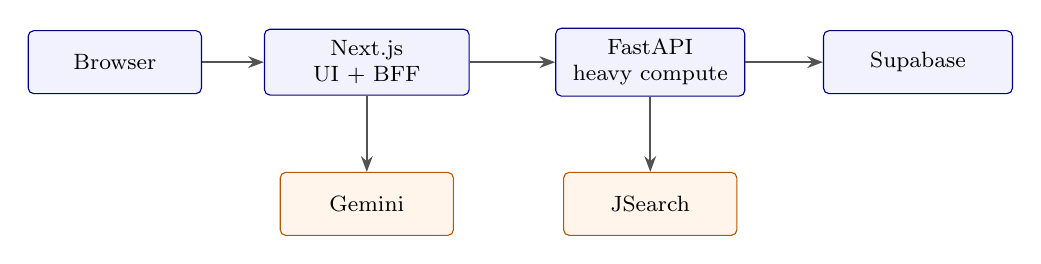
\begin{tikzpicture}[
  x=1cm, y=1cm,
  box/.style={draw=blue!50!black, fill=blue!5, rounded corners=2pt,
              minimum height=8mm, inner sep=4pt, align=center, font=\footnotesize},
  ext/.style={draw=orange!70!black, fill=orange!8, rounded corners=2pt,
              minimum height=8mm, inner sep=4pt, align=center, font=\footnotesize},
  arr/.style={-{Stealth[length=2mm]}, semithick, draw=gray!65!black},
]
  \node[box, minimum width=2.2cm] (browser) at (0,0) {Browser};
  \node[box, minimum width=2.6cm] (next) at (3.2,0) {Next.js\\UI + BFF};
  \node[box, minimum width=2.4cm] (api) at (6.8,0) {FastAPI\\heavy compute};
  \node[box, minimum width=2.4cm] (db) at (10.2,0) {Supabase};

  \node[ext, minimum width=2.2cm] (gem) at (3.2,-1.8) {Gemini};
  \node[ext, minimum width=2.2cm] (js) at (6.8,-1.8) {JSearch};

  \draw[arr] (browser) -- (next);
  \draw[arr] (next) -- (api);
  \draw[arr] (api) -- (db);
  \draw[arr] (next.south) -- (gem.north);
  \draw[arr] (api.south) -- (js.north);
\end{tikzpicture}
\end{center}

\vspace{0.5em}
\begin{center}
\small
\begin{tabularx}{\linewidth}{|>{\bfseries}l|>{\raggedright\arraybackslash}X|>{\raggedright\arraybackslash}X|}
\hline
Path & Used for & Why split \\
\hline
FastAPI & CV upload, job search, fit score, tracker & CPU/API-heavy; service-role DB access \\
\hline
Next.js BFF & Chat stream, cover letter, dashboard nudges & SSE streaming near the UI \\
\hline
Supabase direct & Calendar, simple CRUD & RLS-enforced reads/writes without extra backend hop \\
\hline
\end{tabularx}
\end{center}

\vspace{0.4em}
\noindent\textbf{Trade-off:} Gemini is called from both FastAPI and Next.js --- acceptable for the hackathon; production would centralize AI calls and quotas (see \texttt{system-design.pdf}).

% ===========================================================================
\sectiontitle{4. Supporting Libraries (High Level)}
% ===========================================================================

\begin{center}
\small
\begin{tabularx}{\linewidth}{|l|>{\raggedright\arraybackslash}X|>{\raggedright\arraybackslash}X|}
\hline
\textbf{Area} & \textbf{Choice} & \textbf{Why (one line)} \\
\hline
UI & Tailwind CSS 4, Lucide & Fast, consistent workspace UI \\
\hline
State & TanStack Query & Cache dashboard/tracker; fewer duplicate requests \\
\hline
Tracker UI & @hello-pangea/dnd & Kanban drag-and-drop \\
\hline
Calendar & react-big-calendar & Deadline and interview views \\
\hline
PDF/DOCX & pypdf, python-docx & Server-side CV text extraction \\
\hline
Tests & Vitest (frontend), pytest (backend) & Matches each runtime \\
\hline
\end{tabularx}
\end{center}

% ===========================================================================
\sectiontitle{5. What We Deliberately Did Not Use}
% ===========================================================================

\begin{center}
\small
\begin{tabularx}{\linewidth}{|>{\raggedright\arraybackslash}p{4.8cm}|>{\raggedright\arraybackslash}X|}
\hline
\textbf{Omitted} & \textbf{Reason} \\
\hline
Separate vector DB (Pinecone, Weaviate) & pgvector is enough at hackathon scale \\
\hline
Local LLM / Ollama & Setup friction and inconsistent demo quality \\
\hline
Microservices & One FastAPI app + one Next app covers four pillars \\
\hline
Custom auth server & Supabase Auth covers signup, sessions, JWT for API \\
\hline
\end{tabularx}
\end{center}

% ===========================================================================
\sectiontitle{6. Summary}
% ===========================================================================

\noindent
CareerPilot's stack optimizes for \textbf{one RAG store}, \textbf{live job search}, and \textbf{fast full-stack delivery}: Next.js for UX and streaming, FastAPI for CV/job logic, Supabase for data and vectors, Gemini for AI, JSearch for external listings. Each choice maps to a product requirement --- with a documented scale path (async CV workers, Redis cache, centralized AI gateway) in \textbf{system-design.pdf}.

\vspace{1.2em}
\hrule
\vspace{0.4em}
{\footnotesize\itshape Submission artifact --- \texttt{Docs/submit/stack-report.tex}}

\end{document}
